\documentclass{article}
\usepackage[margin=.9in]{geometry}
\usepackage{xcolor}
\usepackage{amsmath}
\usepackage{amssymb}
\usepackage{float}
\usepackage{listings}
\usepackage{natbib}
\usepackage{booktabs}
\setlength{\parindent}{0pt}
\setlength{\parskip}{\baselineskip}
\definecolor{mycolor}{rgb}{0.1, 0.1, 0.5}
\title{\textcolor{mycolor}{\textbf{{\huge Development and Implementation of a Low-Cost Electrochemistry Lab Kit for Educational Outreach}}}}
\author{Student: Christopher Hunt \\ Mentor: Dr. Kelsey Stoerzinger}
\date{}
\usepackage{graphicx} 
\usepackage{fancyhdr}

\begin{document}
\pagestyle{fancy}
\fancyhf{}
\rfoot{}
\lfoot{Christopher Hunt}
\lhead{Development and Implementation of a Low-Cost Electrochemistry Lab Kit for Educational Outreach}
\rhead{\thepage}
\maketitle

\subsection*{Abstract}
\subsection*{Introduction}
Electrochemical research holds immense potential to address challenges in energy sustainability and environmental conservation. This field encompasses work on renewable energy generation, energy storage, and environmental remediation, among others. A cornerstone for propelling advancements in these areas is educating the next generation of engineers and scientists. However, the significant costs associated with essential instrumentation, coupled with a lack of educational resources, present considerable hurdles.

At the heart of electrochemical research lies the potentiostat, an instrument fundamental to a variety of experimental methods. Commercial potentiostats often retail for over a thousand dollars, a price point that restricts educational opportunities and limits the pursuit of electrochemical innovation.

An increasing number of researchers have leveraged the rising accessibility of affordable microcontrollers, like the Arduino Uno, to develop low-cost potentiostats [Cook 2020]. While these economical devices may not yet match the capabilities of their commercial counterparts, they serve as invaluable educational tools. Still a gap exists between the research and the standardization of design for academic use. Literature explored in this review has shown designs all meeting benchmark testing, however, these projects remain difficult to implement in a high school or undergraduate setting. By introducing electrochemical techniques to students and resource-constrained communities, these low-cost potentiostats facilitate learning and stimulate innovation, despite financial limitations.

\subsection*{Literature Review}
Four potentiostat designs were reviewed: The Meloni Design [Meloni 2016], CheapStat [Rowe 2011], PaqariStat [Cordova-Huaman 2021], and SimpleStat [Butterworth 2019]. These designs will be evaluated against specific criteria that align with our ambition to enhance education and outreach in Electrochemical Engineering. These criteria include: design complexity, functional efficacy, and educational accessibility.

\subsubsection*{Design Complexity}
Potentiostat design complexity is a critical factor that influences both the user experience and the device's functional range. Among the four studied designs, two design approaches are discernible: the Arduino-based designs (the Meloni design and Paqari Stat) and the Integrated Chip (IC) based designs (Cheapstat and Simplestat). Each design's complexity is influenced by the hardware architecture and software implementation.

\subsubsection*{Hardware Architecture}
The Meloni design and the Paqari Stat employ an Arduino Uno microcontroller as the backbone of their design. Their hardware architectures are modular, composed of three primary units: a Digital to Analog Converter (DAC)/signal converter, a control amplifier, and a transimpedance amplifier. This modular design approach can facilitate problem isolation, making it easier to diagnose and resolve hardware issues. However, there are slight differences between these two designs; while the Meloni design utilizes a counter electrode to measure output current, the Paqari Stat uses the working electrode for this purpose. This difference might impact the overall measurement accuracy, stability, and noise performance of the system. 

On the other hand, Cheapstat and Simplestat are centered around a surface mount IC microcontroller, a more compact and integrated approach. This kind of architecture results in reduced size and possibly lower power consumption, making these designs more suitable for field applications. However, this integrated design approach could pose challenges in terms of self-assembly and troubleshooting.

\subsubsection*{Software Implementation}
The software for the Arduino-based designs (Meloni and Paqari Stat) is programmed within the Arduino itself. Software development using the Arduino is based on C++, a widely used language that provides good accessibility for non-specialists or beginners. While the Meloni design relies solely on using the Arduino for it's software, the Paqari Stat goes a step further by incorporating a smartphone-based app. While using an existing application may improve user interaction it may reduce the educational benefits of the project.

In contrast, Cheapstat and Simplestat require assembly language coding to program their hardware. Assembly language, a low-level language, allows direct hardware control and optimization but comes at the cost of complexity. Understanding and programming in assembly language can be a challenging task, especially for beginners or non-specialists. This could limit the accessibility and adaptability of these designs to specific experimental setups or novel applications.

For the Meloni design, the hardware and software engineering decisions for the design were clearly explained, making it the design best suited for implementation in an educational context. While, for PaqariStat, Cheapstat, and Simplestat, the hardware design is not well-documented. This lack of clarity could pose significant challenges during self-assembly, especially for users with limited hardware experience. 

Design complexity varies significantly among the four potentiostat designs studied. The Arduino-based designs are characterized by a more modular hardware architecture, user-friendly software. On the contrary, the IC-based designs have more integrated architectures, more complex software, and require more detailed assembly documentation. The choice between these design routes will largely depend on the user's technical skills, application requirements, and available resources.

\subsubsection*{Functional Efficacy}
The functional efficacy of a potentiostat design is defined by its ability to deliver accurate and reliable measurements under various experimental conditions. Each of the four potentiostat designs - the Meloni design (2016), Cheapstat (2011), Paqari Stat (2021), and Simplestat (2019) - was evaluated for their efficacy based on their performance in Cyclic Voltammetry (CV) tests using a standard potassium ferricyanide experiment.

The Meloni design has demonstrated high functional efficacy as its performance closely matched the expected results from the literature. The design follows a three-stage architecture, utilizing an 8-bit Pulse Width Modulation (PWM) signal for control, which may influence the accuracy of the results. However, it should be noted that this design is limited to performing only CV, limiting its applicability to a narrower range of electrochemical experiments. The effect of these design choices on the device's performance in a wider range of experimental conditions is an area that warrants further exploration. The voltage range of the CV scan is fixed at -1v to +1v.

The Paqari Stat demonstrated positive results, with the device's performance falling within acceptable margins when tested against lab-grade equipment. This is an encouraging indication of its functional efficacy. Like the Meloni design, it is based on an Arduino microcontroller and follows a similar three-stage hardware architecture. The Paqari Stat, however, uses the working electrode to measure output current, unlike the Meloni design, which uses a counter electrode. This difference in design choice might have an impact on the comparative functional efficacy of the two designs, though further investigation is required to confirm this.

The CheapStat performed it's benchmark testing using a potassium ferricyanide based experiment as well. The article states that the ferricyanide redox response forms the characteristic ``duck'' shape expect from the experiment. This was conducted using a commercial made reference electrode and a homemade reference, demonstrating close agreemnt when observing the reaction. The device was then used to perform analysis of acetaminophen content in over the counter medication and measurements of arsenic in water. These results show great promise in the efficacy of DIY potentiostat designs.

The Simplestat's performance was also tested against a potassium ferricyanide solution, yielding positive results. Like the Cheapstat, the Simplestat utilizes a surface mount IC microcontroller and is designed around a printed PCB. The Simplestat's design incorporates an 8-bit DAC and a 10-bit Analog to Digital Converter (ADC), allowing for a CV range of -0.6v to 0.6v. These design choices might contribute to the observed efficacy but, as with the Cheapstat, a more detailed elaboration of the testing parameters and comparative performance would enhance understanding of the design's efficacy.

The functional efficacy of each potentiostat design appears promising based on the described CV testing. The efficacy of these designs across a broader range of electrochemical experiments beyond CV would benefit this area of research.

\subsubsection*{Educational Accessibility}
Educational accessibility is a key consideration when assessing these potentiostat designs, particularly in terms of their suitability for teaching environments like undergraduate laboratories. This dimension encompasses the ease of understanding the device's operation, the clarity of its assembly instructions, and the feasibility of using it as a teaching tool to elucidate fundamental electrochemical principles.

The Meloni design, with its Arduino-based approach, offers a relatively straightforward design and software implementation. It relies on a commonly used Arduino Uno microcontroller, an 8-bit signal for control, and a three-stage hardware design, all of which are concepts that are relatively easy to grasp for undergraduate students. The depth of explaination of the hardware's design by Meloni makes it the clearest to implement.

Like the Meloni design, Paqari Stat utilizes an Arduino-based approach, making it comparatively more accessible for educational use. The addition of a smartphone app for controlling the potentiostat makes troubleshooting errors between the hardware and software more difficult to fix. This app could also act as a 'black box', obscuring the underlying processes and impeding students from fully understanding the potentiostat's operation. While this design seems as promising as the Meloni design in terms of educational potential, the role of the smartphone app in an educational setting requires further exploration.

The Cheapstat, with its surface mount IC microcontroller and assembly language coding, presents a more challenging approach for undergraduate students. Assembly language, being a low-level language, provides deeper control over hardware but at the cost of complexity and a steep learning curve. Furthermore, the hardware design is not well-documented, which can cause further obstacles to understanding and replicating the design. While Cheapstat might be more appropriate for graduate students or practicing electrochemists who seek a cost-effective field potentiostat, its educational accessibility for undergraduate students seems limited.

Similar to Cheapstat, SimpleStat employs a surface mounted IC microcontroller and assembly language coding. This results in a higher level of opacity in both hardware and software design, which may present significant challenges for undergraduate students with limited programming and hardware experience. Consequently, it appears more suitable for advanced users such as graduate students or professional electrochemists.

In terms of educational accessibility, the Arduino-based potentiostats (Meloni and Paqari Stat) seem more approachable for undergraduate students due to their relative simplicity and familiar software implementation. The additional smartphone interface of the Paqari Stat could be a double-edged sword, simultaneously promoting engagement while potentially limiting understanding of underlying processes. In contrast, the IC-based designs (Cheapstat and Simplestat) present higher complexity, which might pose substantial challenges for students but offer potentially richer learning experiences for more advanced users. Further research, with a focus on user experience in a real educational setting, could provide valuable insights into the educational accessibility of these designs.


\subsection*{Methodology}
This research undertakes an examination, construction, and testing of various Arduino-based potentiostat designs. After examining several designs, we focused our attention on the Meloni Design due to its detailed circuit layout and ease of replication. We further enhanced this design by incorporating a 10-bit digital-analog converter to achieve a higher resolution control signal. Due to the limitations of this DIY potentiostat, specific component choices and layout may require adjustments to accurately provide data for our use case. The design will be constructed to properly detect the current generated from a Ferricyanide/Ferrocyanide redox reaction during a cyclic voltammetry (CV) experiment, the common benchmark test for the articles examined in our literature review. The methodology section thus elaborates on the research design, data collection, data analysis processes, and the limitations encountered in the study.

A comparative analysis of Arduino-based designs was performed. Arduino microcontrollers are known for their affordability and ease of implementation. From our literature review, it was determined that the hardware design will reflect the design choices made in The Meloni Design. This was chosen based on its detailed schematic and commonality in the potentiostat designs literature. This design, however, may require adjustments to the control signal and several component values to be operable within our research's specific test case.

The Meloni Design is comprised of 7 stages (fig. 1).
\begin{enumerate}
    \item Software-generated Pulse Width Modulated (PWM) control signal
    \item Hardware filtering of control signal
    \item Control signal biasing
    \item Potentiostat control amplifier
    \item Current to voltage conversion
    \item Output signal buffer
    \item Output signal software processing
\end{enumerate}

\begin{figure}[H]
    \centering
    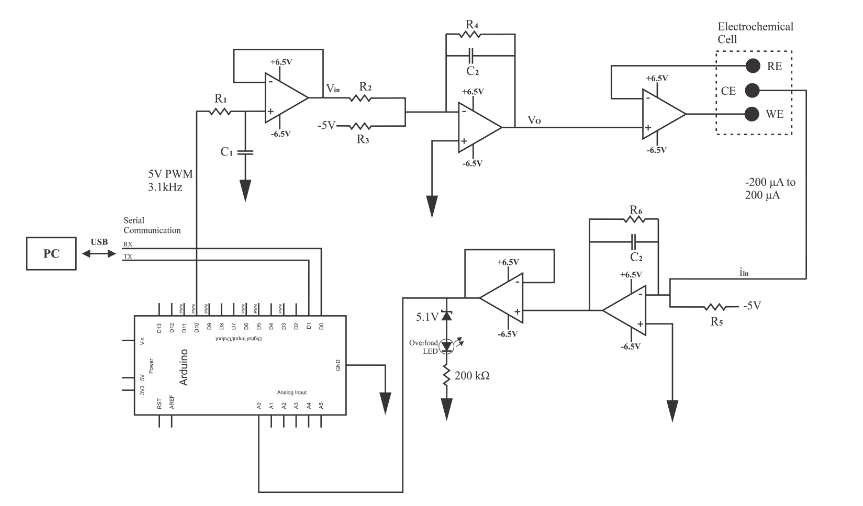
\includegraphics[width=.7\linewidth]{meloni_design.png}
    \caption{Meloni Design}
\end{figure}

The electrochemical reaction to be studied is a ferricyanide/ferrocyanide redox reaction. This reaction will first be conducted using a BioLogic VSP-300 potentiostat using the EC-Lab software. A CV will be produced using a potential window from 0 to 0.5 volts, with scan rates of 20, 50, and 100 mV/s. This benchmark testing will provide an expected current range of the redox reaction. 

There are three design components that are being adjusted from the Meloni Design. First, we changed how the control signal is generated. The Meloni Design uses a single PWM pin from the Arduino in combination with an RC filter and an op-amp in an integrator configuration to produce the control signal for the CV. For our design, we chose to use a 10-bit Digital-Analog Converter (DAC) using an R2R ladder. This offers two benefits: first, it offers greater resolution for the control signal - 10-bit precision instead of 8-bit with the PWM design. Second, the R2R ladder is a fundamental circuit design used in entry-level electrical engineering coursework, whereas the PWM design may be considered more advanced. Second, we chose to swap the connections between the working electrode (WE) and the counter electrode (CE). This design decision was made with consultation from a BioLogic representative who claimed that since we are concerned about the current through the working electrode, it is assumed that measuring the current directly through it is the optimal design solution. Third, we must alter the values of the current to voltage converter. We will use the benchmark testing current maximum and minimum values to calculate the appropriate resistor and capacitor values for this circuit.

The modifications to the original Meloni Design were made in line with theoretical circuit analysis techniques. The use of an R2R ladder and the need for future students to perform circuit analysis to attenuate component values offer a greater learning opportunity for students.

We are adopting a twofold data collection process. First, we will collect circuit output measurements to validate each stage of the design. This ensures that the hardware is outputing the expected values in each stage of the hardware before conducting any electrochemical experiments. Next, we will perform the ferri/ferrocyanide experiment. The current from the working electrode will be converted to a voltage between 0-5V. The data collected will be transfered to a PC and then processed using python.

Our research, while thorough, encounters certain limitations. The resolution of the cyclic voltammetry control signal and the analog input detector is 4.88 millivolts, which may not be sufficient for some highly sensitive applications. In addition, aligning the output current to a 0-5V scale presents a challenge as it's not entirely accurate. The signal conversion hardware assumes a maximum and minimum current, which could be variable. If the current is outside this range, the sensor either outputs 0 or 1023, meaning the measurements could be clipped or skewed.

This research presents a comprehensive methodology to assess, improve, and compare Arduino-based potentiostat designs. While there are some limitations, the study leverages the strengths of existing designs, particularly the Meloni Design, and contributes valuable enhancements to this field. Further studies can build on these findings, optimizing and addressing the identified limitations.

\subsection*{Results}
\subsection*{Discussion}
\subsection*{Conclusion}

In this literature review, we explored four distinctive low-cost potentiostat designs for educational outreach: The Meloni design, CheapStat, PaqariStat, and SimpleStat. We evaluated them based on their design complexity, functional efficacy, and educational accessibility.

From the perspective of design complexity, the Arduino-based designs (Meloni and Paqari Stat) emerged as user-friendly options due to their modular hardware architectures and high-level software.The IC-based designs (Cheapstat and Simplestat), although more integrated and possibly energy efficient, presented challenges in self-assembly and required more detailed assembly documentation. The Meloni design provided the most detailed explaination for implementation of the four. 

As for functional efficacy, all four designs showcased promising results based on the CV tests. However, given the variation in the level of detail provided and the range of electrochemical experiments, more comprehensive testing and documentation are necessary for a thorough comparison and understanding of their functional capabilities.

In terms of educational accessibility, the Arduino-based designs (Meloni and Paqari Stat) appeared more suited for undergraduate students, whereas IC-based designs (Cheapstat and Simplestat), despite their higher complexity, might offer a richer learning experience for more advanced users.

While this review provides a comprehensive exploration of these four low-cost potentiostat designs, the final selection would inevitably depend on the users' specific needs and the educational environment they will be deployed in. Further hands-on exploration and user experience studies could augment the understanding of these designs' real-world applicability and potential. It is our hope that this review aids in identifying suitable low-cost potentiostat designs for educators and researchers striving to democratize and innovate electrochemical education. We are enthusiastic about the promise that these low-cost designs hold for bridging the gap between electrochemical research and educational outreach.

However, it is clear that more work is needed to standardize these designs for academic use. The community should continue pushing towards producing low-cost, reliable, and accessible potentiostat designs, thereby accelerating learning and innovation in the field of electrochemistry.
\subsection*{References}
Butterworth A, Corrigan DK, et al. (2019) Electrochemical detection of oxacillin resistance with SimpleStat: a low cost integrated potentiostat and sensor platform. \emph{Analytical Methods.} Issue 14. 

Cook J (2020). SIMstat: Hardware Design Considerations for Implementing a Low-Cost, Portable Potentiostat. \emph{Unpublished Bachelor's Thesis}. Oregon State University

Cordova-Huaman AV, Jauja-Ccana VR, et al. (2021) Low-cost smartphone-controlled potentiostat based on Arduino for teaching electrochemistry fundamentals and applications.\emph{Heliyon}, Volume 7, Issue 2. 

Meloni, GN (2016). Building a Microcontroller Based Potentiostat: A Inexpensive and Versatile Platform for Teaching Electrochemistry and Instrumentation. \emph{Journal of Chemical Education} 93(7), 1320-1322. 

Rowe AA, Bonham AJ, et al. (2011) CheapStat: An Open-Source, ‘‘Do-It-Yourself’’ Potentiostat for Analytical and Educational Applications. \emph{PLoS ONE} 6(9).

\end{document}